\documentclass{article}
\usepackage[UTF8]{ctex}

\usepackage{amsmath}        %数学公式
\usepackage{amssymb}
\usepackage{cases}          %联立编号
\usepackage{cite}           %引用

\usepackage{graphicx}       %插入图片
\usepackage{float}          %设置图片浮动位置
\usepackage{subfigure}      %插入多图时用子图显示

\usepackage{listings}
\usepackage{xcolor}

\usepackage{anyfontsize}    %解决一个奇怪的字体大小报错问题
\usepackage{fancyhdr}       %页眉、页脚、页码
\usepackage[a4paper, margin=1in]{geometry}    %纸张大小
\usepackage{longtable}

\lstset{
    basicstyle          =   \sffamily,          % 基本代码风格
    keywordstyle        =   \bfseries,          % 关键字风格
    commentstyle        =   \rmfamily\itshape,  % 注释的风格,斜体
    stringstyle         =   \ttfamily,  % 字符串风格
    flexiblecolumns,                % 别问为什么,加上这个
    numbers             =   left,   % 行号的位置在左边
    showspaces          =   false,  % 是否显示空格,显示了有点乱,所以不现实了
    numberstyle         =   \zihao{-5}\ttfamily,    % 行号的样式,小五号,tt等宽字体
    showstringspaces    =   false,
    captionpos          =   t,      % 这段代码的名字所呈现的位置,t指的是top上面
    frame               =   lrtb,   % 显示边框
}

\lstdefinestyle{Python}{
    language        =   Python, % 语言选Python
    basicstyle      =   \zihao{-5}\ttfamily,
    numberstyle     =   \zihao{-5}\ttfamily,
    keywordstyle    =   \color{blue},
    keywordstyle    =   [2] \color{teal},
    stringstyle     =   \color{magenta},
    commentstyle    =   \color{red}\ttfamily,
    breaklines      =   true,   % 自动换行,建议不要写太长的行
    columns         =   fixed,  % 如果不加这一句,字间距就不固定,很丑,必须加
    basewidth       =   0.5em,
}

\newcommand\f[2]{\frac{#1}{#2}}
\newcommand\pf[2]{\frac{\partial#1}{\partial#2}}
\newcommand\df[2]{\dfrac{#1}{#2}}
\newcommand\pdf[2]{\dfrac{\partial#1}{\partial#2}}
\newcommand\zsin[1]{\frac{e^{i#1}-e^{-i#1}}{2i}}
\newcommand\zdsin[1]{\dfrac{e^{i#1}-e^{-i#1}}{2i}}
\newcommand\zcos[1]{\frac{e^{i#1}+e^{-i#1}}{2i}}
\newcommand\zdcos[1]{\dfrac{e^{i#1}+e^{-i#1}}{2i}}
\newcommand\zline[1]{#1-\overline{#1}}
\newcommand\dg[2]{#1^{\circ}#2'}

\setlength{\headheight}{16pt}
\pagestyle{fancy}
\fancyhf{}

\title{\bf\huge 一二维随机游走的偏移量}
\author{Jerry}
\date{\today}
\pagenumbering{arabic}

\begin{document}

\fancyhead[L]{Jerry}
\fancyhead[C]{一二维随机游走的偏移量}
\fancyhead[R]{概率论与数理统计-唐宏岩}
\fancyfoot[C]{\thepage}

\maketitle

\section{从作业中赌博的例子谈起}

在第二周的作业中,有这样一个题目:

\emph{*10.某人参与一个游戏,每次输赢$1$元,赢的概率为$p>0$,且每次游戏之间相互独立,
假设初始资金为$k$元,输光或者资金达到$n$元离场($n>k$).}

\emph{(1. )此人输光离场的概率为多少?}

\emph{(2. )如果$p\leq0.5$,当$n\to\infty$时,求其输光离场概率的极限.}

答案也很容易得出:

\emph{(1. )}

\emph{设拥有$k$元时,输光离场的概率为$p_k$。}

\emph{在第一次参与后有$p$的概率变成$k+1$元,
有$1-p$的概率变成$k-1$元,可以得到递推关系式$$p_k=pp_{k+1}+(1-p)p_{k-1}$$}

\emph{对这个式子处理得到}

\emph{$$p_n-p_0=(p_1-p_0)((\frac{1-p}{p})^{n-1}+(\frac{1-p}{p})^{n-2}+...+(\frac{1-p}{p})^{0})$$}

\emph{(1. a. )$p\neq0.5$}

\emph{$$p_n-p_0=(p_1-p_0)(\frac{1-(\frac{1-p}{p})^n}{1-\frac{1-p}{p}})\text{,}p_k-p_0=(p_1-p_0)(\frac{1-(\frac{1-p}{p})^k}{1-\frac{1-p}{p}})$$}

\emph{两式相除,得到$$\frac{p_n-p_0}{p_k-p_0}=\frac{1-(\frac{1-p}{p})^n}{1-(\frac{1-p}{p})^k}$$}

\emph{考虑到$p_{n}=0,p_0=1$,故$$p_k=1-\frac{1-(\frac{1-p}{p})^k}{1-(\frac{1-p}{p})^n}$$}

\emph{(1. b. )$p=0.5$}

\emph{$$p_n-p_0=n(p_1-p_0)\text{,}p_k-p_0=k(p_1-p_0)$$}

\emph{两式相除,得到$$\frac{p_n-p_0}{p_k-p_0}=\frac{n}{k}$$}

\emph{考虑到$p_{n}=0,p_0=1$,故$$p_k=1-\frac{k}{n}$$}

\emph{(2. )}

\emph{在$p\leq0.5$时,}

\emph{(2. a. )$p<0.5$}

\emph{$$\lim_{n\to\infty}p_k=1-\lim_{n\to\infty}\frac{1-(\frac{1-p}{p})^k}{1-(\frac{1-p}{p})^n}=1-0=1$$}

\emph{(2. b. )$p=0.5$}

\emph{$$\lim_{n\to\infty}p_k=1-\lim_{n\to\infty}\frac{k}{n}=1-0=1$$}

可以看出,这个赌徒最终会血本无归。

那有没有一种可能让这个赌徒赢过庄家呢?

我们考虑一场“公平”的赌博,即$p=0.5$,$p_k=1-\frac{k}{n}$。值得一提的是,此时
存在一种的赢过庄家的可能,即让自己的钱比赌场主的钱更多:如果假设赌徒的资金为$a$,
赌场主的资金为$b$,则赌场主破产的概率为$\frac{a}{a+b}$。\cite{WikiRW}

\section{如果赌徒的钱可以为负数}

在这样的推广下,我们假设这个赌徒和庄家的钱可以为负数(或假设赌徒和庄家的赌资都是无穷多的),重新考虑这个问题。
我们尝试计算考虑$k$次赌博后,这个赌徒的收益$S_n$的一些性质。

我们可以将这个赌博的过程数学抽象为一个一维随机游走模型:

\emph{存在独立的随机变量$X_1,X_2,\dots,X_n$,其中每个变量的值为$1$或$-1$,
任一值的概率均为50\%。定义$n$次游走后的位置为$S_n=\sum_{0}^{n}X_i(n\in Z)$,
并令$S_0$=0。}

计算$n$次游走后的位置的概率分布函数:

$$P(S_n=k)=\sum_{i=1}^{n}C_{n}^{\df{n+k}{2}}\left(\df{1}{2}\right)^{\df{n+k}{2}}\left(\df{1}{2}\right)^{\df{n-k}{2}}=\df{1}{2^n}\sum_{i=1}^{n}C_{n}^{\df{k+n}{2}}$$

我们计算$S_n$和$S_n^2$的期望:

\begin{equation*}
    \begin{aligned}
        E(S_n) & =\sum_{i=1}^{n}E(X_i)=0\\
        E(S_n^2) & =\sum_{i=1}^{n}E(X_i^2)+2\sum_{1\leq i<j\leq n}^{}E(X_iX_j)=n\\
    \end{aligned}
\end{equation*}

从$E(S_n^2)=n$可以猜测$|S_n|$应该是$\sqrt{n}$量级。事实上,可以得到\cite{RW1D}:

\begin{equation*}
    \begin{aligned}
        & |S_n|=\df{2}{\sqrt{\pi}}\df{\Gamma(J+\df{1}{2})}{\Gamma(J)}=\df{(2J-1)!!}{(2J-2)!!}\\ \\
        & \text{其中,}J=\left\{
        \begin{aligned}
            & \df{n}{2}\text{\ \ \ \ \ \ \ \ \ }&n \text{为偶数}\\
            & \df{n+1}{2}&n \text{为奇数}\\
        \end{aligned}
        \right.
    \end{aligned}
\end{equation*}

对这个式子进行展开,可以得到:$$|S_n|=\sqrt{\df{2n}{\pi}}(1\mp\df{1}{4n}+\df{1}{32n^2}\pm\df{5}{128n^3}-\df{21}{2048n^4}\mp\dots)$$

对于较大的$n$,则只取第一项,即$$|S_n|\sim\sqrt{\df{2n}{\pi}}$$

事实上,在$n$非常大时,这一分布可以近似为正态分布

$$P(S_n=k)=\df{1}{\sqrt[]{2\pi n}}e^{-\df{1}{2}\left(\df{k}{\sqrt[]{n}}\right)^2}=\df{1}{\sqrt[]{2\pi n}}e^{-\df{k^2}{2n}}$$

对这个正态分布积分同理可得:$$E(|S_n|)=\int_{-\infty}^{\infty}|x|\cdot\df{1}{\sqrt[]{2\pi n}}e^{-\df{x^2}{2n}}dx=\sqrt{\df{2n}{\pi}}$$

这意味着这个随机游走的期望位置为原点,但是期望的偏移量为$\sqrt{\df{2n}{\pi}}$。

回到原来的赌徒问题,也就是说这个赌徒在经过$n$次赌博后,期望为不赚不亏,但是预期的
收益/亏损为$\sqrt{\df{2n}{\pi}}$元。

\section{一个醉汉在沿着格子走路}

我们将这个一维的随机游走问题扩展到二维,我们假设有一位醉汉,在地面上,每次向
前、后、左、右四个方向随机走一步,并且每次走的概率均为$\frac{1}{4}$,
我们考虑这个醉汉的随机游走过程。

我们可以将这个醉汉的随机游走过程数学抽象为一个二维随机游走模型:

\emph{存在独立的随机变量$D_1,D_2,\dots,D_n$,其中每个变量的值为$(1,0),(-1,0),(0,1),(0,-1)$,
任一值的概率均为25\%。定义$n$次游走后的位置为$S_n=\sum_{0}^{n}D_i(n\in Z)$,
并令$S_0$=0。}

在这个问题中,$D_i$是一个二维向量,它表示在二维空间的随机游走。每一步的游走结果是向
正$x$轴方向移动一单位、向负$x$轴方向移动一单位、向正$y$轴方向移动一单位、或者向负$y$轴
方向移动一单位,每个方向的概率都是25\%。所以实际上,我们有两个独立的一维随机游走:一个
在$x$轴上,一个在$y$轴上。

让我们定义两个独立的随机变量$X_i$和$Y_i$,分别表示第$i$次移动在x轴和y轴上的位置变化。
每个随机变量可以取值$1$或$-1$,概率为50\%(因为在$D_i$中向任一轴的正方向或负方向移动
的概率总和是50\%)。

我们感兴趣的是$S_n$,即经过$n$次移动后的总位移向量,它的每个分量可以表示为$X = \sum_{i=1}^{n} X_i$和$Y = \sum_{i=1}^{n} Y_i$。

由于$X_i$和$Y_i$都是独立同分布的随机变量,$X$和$Y$的分布都是中心在原点的随机游走。

现在我们需要计算经过$n$次移动后,游走者距离原点的期望距离。我们定义这个距离$|D_n|$是随机变量$X$和$Y$的欧几里得距离:

$$|D_n|=\sqrt{X^2 + Y^2}$$

同一维随机游走,我们可以得到:$E[X^2]=\text{Var}(X)=n$、$E[Y^2]=\text{Var}(Y)=n$

所以:

$$E(D^2)=E[X^2+Y^2]=E[X^2]+E[Y^2]=2n$$

从$E(D_n^2)=2n$可以猜测$|S_n|$应该是$\sqrt{n}$量级。事实上:

对于大的$n$,我们可以使用中心极限定理来近似$X$和$Y$的分布为正态分布。在这种情况下,
由于$X$和$Y$的方差都是$n$,并且$X^2 + Y^2$的期望是$2n$,我们可以说$X^2 + Y^2$近似为
一个卡方分布,其自由度是$2$,因为有两个独立的分量$X$和$Y$。卡方分布的期望值等于其自由度,
同理可以得到$E(X^2+Y^2)$是$2n$。

我们难以计算出$E(|D_n|)$,只能通过数值模拟来得出大概的值。同时,我们也可以通过计算
$E(\sqrt{D_n^2})$的来得到$E(|D_n|)$的量级为$\sqrt{n}$。

但是,好消息是,对于另一个平面上行走的醉汉,他的期望距离是可以很轻松的求出的。

\section{当醉汉向任意方向迈步时}

我们考虑一个新的醉汉,他向$[0,2\pi)$的任意方向迈步,每次迈步的长度都是$1$,我们考虑这个醉汉的随机游走过程。\cite{RW2D}

\emph{存在独立的随机变量$\theta_1,\theta_2,\dots,\theta_n$,其中每个变量的取值范围为$[0,2\pi)$,
定义$n$次游走后的位置为$z_n=\sum_{j=0}^{n}e^{i\theta_j}(n\in Z)$,并令$z_0$=0。}

在平面中,我们考虑具有随机方向的二维向量的总和。则在$N$步后,这个醉汉的位置$z$可以由下式给出:$$z=\sum_{j=1}^{N}e^{i\theta_j}$$

这个值有绝对平方

\begin{equation*}
    \begin{aligned}
        |z|^2 & =\sum_{j=1}^{N}e^{i\theta_j}\sum_{k=1}^{N}e^{-i\theta_k}\\
              & =\sum_{j=1}^{N}\sum_{k=1}^{N}e^{i(\theta_j-\theta_k)}\\
              & =N+\sum_{j\neq k}^{N}e^{i(\theta_j-\theta_k)}\\
    \end{aligned}
\end{equation*}

每一步在任何方向上的可能性相同,位移是均值相同且为0的随机变量,则他们的差值也是均值为0的随机变量。

故$E(e^{i(\theta_j-\theta_k)})=0$,因此$|z|^2=N$,即$|z|=\sqrt{N}$。

\section{然后编一个程序进行验证}

\subsection{一维随机游走}

通过python程序计算得到的结果如下:

E(|X|) of data: 2618

Expected value of E(|X|): 2523.13252202016

(E(|D|)-Expected\_E(x))/Expected\_E(x) of data: 0.037599086513253624

可以看出试验结果与预期符合较好。

\begin{figure}[H]
    \centering
    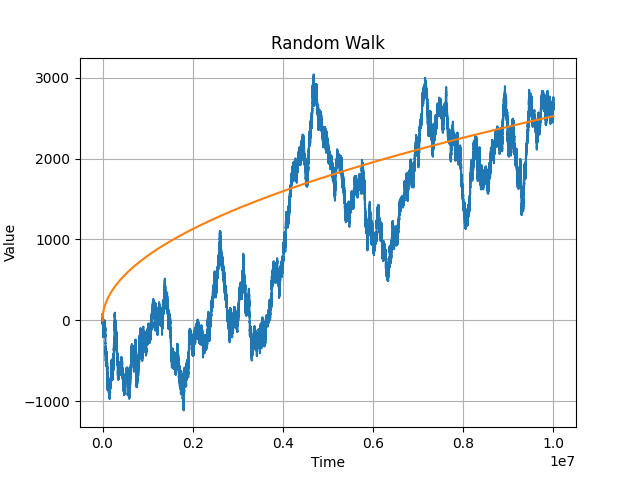
\includegraphics[width=0.8\textwidth]{img/Figure_1D.png}
    \caption{一维随机游走}
\end{figure}

源代码如下:

\lstinputlisting[
    style       =   Python,
    caption     =   {\bf simulation1D.py},
    label       =   {1}
]{code/simulation1D.py}

\subsection{二维随机游走-醉汉在格子上走}

通过python程序计算得到的结果如下:

E(|D|) of data: 2621.957284167688

E(|D|)/sqrt(n) of data: 0.8291356945639234

可以大致认为这个系数为0.829,即$$E(|D|)\approx0.829\sqrt{n}$$

\begin{figure}[H]
    \centering
    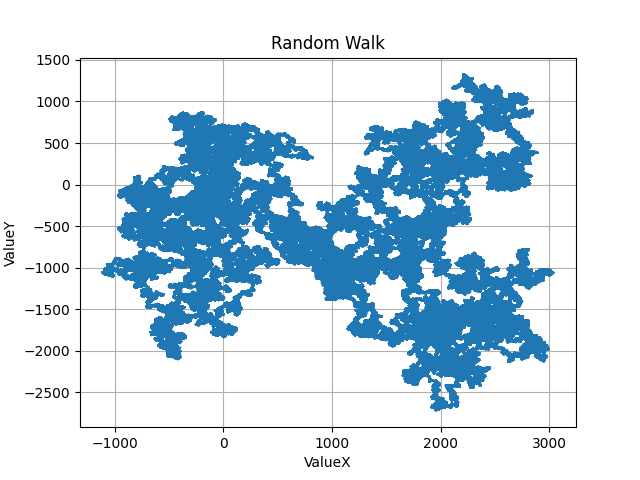
\includegraphics[width=0.8\textwidth]{img/Figure_2D1.png}
    \caption{二维随机游走-醉汉在格子上走}
\end{figure}

源代码如下:

\lstinputlisting[
    style       =   Python,
    caption     =   {\bf simulation2D.py},
    label       =   {2}
]{code/simulation2D1.py}

\subsection{二维随机游走-醉汉在平面上走}

通过python程序计算得到的结果如下:

E(|D|) of data: 3182.458629509072
Expected value of E(|D|): 3162.2776601683795
(E(|D|)-sqrt(n))/E(|D|) of data: 0.0063413139619683

可以看出试验结果与预期符合较好。

\begin{figure}[H]
    \centering
    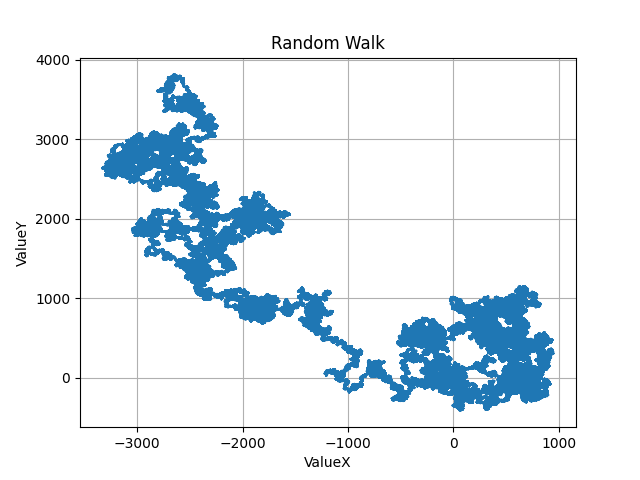
\includegraphics[width=0.8\textwidth]{img/Figure_2D2.png}
    \caption{二维随机游走-醉汉在平面上走}
\end{figure}

源代码如下:

\lstinputlisting[
    style       =   Python,
    caption     =   {\bf simulation2D2.py},
    label       =   {3}
]{code/simulation2D2.py}

\section{最后对论文进行一个总结}

在这个小论文中,我通过数学分析和计算机模拟的方法,从赌徒的例子出发,推广到一维、二维随机游走的问题,
研究了一维和二维随机游走的期望偏移量。最终得到了一维随机游走的期望偏移量为$\sqrt{\f{2n}{\pi}}$,
二维非网格随机游走的期望偏移量为$\sqrt{n}$,二维网格随机游走的期望偏移量大致为$0.829\sqrt{n}$。但是,
在研究中仅限于一维和二维的情况,对于更高维度的情况,我并没有进行研究,这也是一个值得探讨的问题。

% plain(参考文献的条目编号是按照字母的顺序)
% unsrt(参考文献的条目编号是按照引用的顺序)
% alpha(参考文献的条目编号是按照作者名字和出版年份的顺序)
% abbrv(缩写格式)

\bibliographystyle{unsrt}
\bibliography{cite.bib}

\end{document}